

\documentclass[12pt]{article}
\usepackage{amsmath}
\RequirePackage{hyperref}
\usepackage{graphicx}
\usepackage{booktabs}
\usepackage{multirow}
\usepackage{makecell}

\title{Supplemental Material - Assessing 16S marker gene survey data analysis methods using mixtures of human stool sample DNA extracts.}
\author{ND Olson et. al}

\begin{document}
\maketitle

\section*{Titration Series Validation and Correction}
\subsection*{Methods}
To increase confidence in the expected values used in our assessment framework we validated the proportion of unmixed samples measured by the 16S rRNA marker-gene sequencing assay.
To correct for observed deviation from our mixture design we estimated the proportion of unmixed POST in the titrations using the 16S rRNA sequencing data.

\paragraph*{Volumetric Mixing Validation}

qPCR was used to validate volumetric mixing and check for differences in
the proportion of prokaryotic DNA across titrations
(Fig. \ref{fig:titrationValidation}). To ensure the two-sample titrations
were volumetrically mixed according to the mixture design,
independent ERCC plasmids were spiked into the unmixed PRE and
POST samples \cite{baker2005external} (NIST SRM SRM 2374) (Table
\ref{tab:erccTable}). The ERCC plasmids were resuspended in 100
\(\mu L\) tris-EDTA buffer and 2 \(\mu L\) of resuspended plasmids was
spiked into the appropriate unmixed sample. Plasmids were spiked into
unmixed PRE and POST samples with normalized DNA concentration of
12.5 \(ng/\mu L\). POST sample ERCC plasmid abundance was quantified
using TaqMan gene expression assays (FAM-MGB, Catalog \# 4448892,
ThermoFisher) specific to each ERCC plasmid and TaqMan Universal
MasterMix II (Catalog \# 4440040, ThermoFisher Waltham, MA USA).
qPCR assays were perfomed in triplicate using the QuantStudio
Real-Time qPCR (ThermoFisher). ERCCs were also spiked into PRE
samples but were not used to validate volumetric mixing as PRE sample
proportion differences were too small for qPCR quantification.
The expected difference for the entire range of PRE concentrations
is 1 \(C_t\).


To check for differences in the proportion of bacterial DNA in the PRE
and POST samples, bacterial DNA concentration in the titrations was quantified
using the Femto Bacterial DNA quantification kit (Zymo Research, Irvine
CA). All samples were run in triplicate along with an in-house \emph{E.
coli} DNA \(log_{10}\) dilution standard curve. Three concentrations were used
for the in-house standard, 20 ng/ul, 2ng/ul, and 0.2 ng/ul,
with 91.49 efficiency and 0.999 \(R^2\). qPCR assays were
performed using the QuantStudio Real-Time qPCR (ThermoFisher).
Amplification data and Ct values were exported as tsv files using
QuantStudio™ Design and Analysis Software v1.4.1. Statistical analysis
was performed on the exported data using custom scripts in R \cite{R}.
The qPCR data and scripts used to analyze the data are available at
\url{https://github.com/nate-d-olson/mgtst_pub}.


The following linear model \eqref{eq:thetaInf} was used to infer the
proportion of prokaryotic DNA, \(\theta\), in each titration. Where
\(\textbf{Q}_{i}\) is a vector of titration \(i\) feature relative
abundance estimates and \(\textbf{Q}_{pre}\) and \(\textbf{Q}_{post}\)
are vectors of feature relative abundance estimates for the unmixed PRE
and POST samples. Feature relative abundance estimates were calculated
using a negative binomial model.

\begin{equation}
  \textbf{Q}_{i} = \theta_i (\textbf{Q}_{post} -\textbf{Q}_{pre}) + \textbf{Q}_{pre}
  \label{eq:thetaInf}
\end{equation}

To fit the model and prevent uninformative and low abundance features
from biasing \(\theta\) estimates, only features meeting the following
criteria were used. To improve feature level model fit, features had to be observed in at least 14 of the 28 total titration PCR replicates (4 replicates per 7 titrations.)
To increase confidence in PRE and POST abundance estimates the features were present in either all four or none of the PRE and POST PCR replicates.
Finally, to eliminate uninformative features with no change in abundance across titrations only features with greater than 2-fold difference in relative abundance between the PRE and POST samples were used.

16S rRNA sequencing count data is known to have a non-normal
mean-variance relationship resulting in poor model fit for standard
linear regression \cite{McMurdie2014}. Generalized linear models
provide an alternative to standard least-squares regression. The above
model is additive and therefore \(\theta_i\) cannot be directly inferred
in log-space. To address this limitation, we fit a model to \eqref{eq:thetaInf}
using standard least-squares regression and obtained non-parametric 95 \%
confidence intervals for the \(\theta\) estimates by bootstrapping with 1000
replicates. Bootstrapping was performed by resampling informative features, defined above, by subject.

\subsection*{Results}

\begin{figure}
\centering
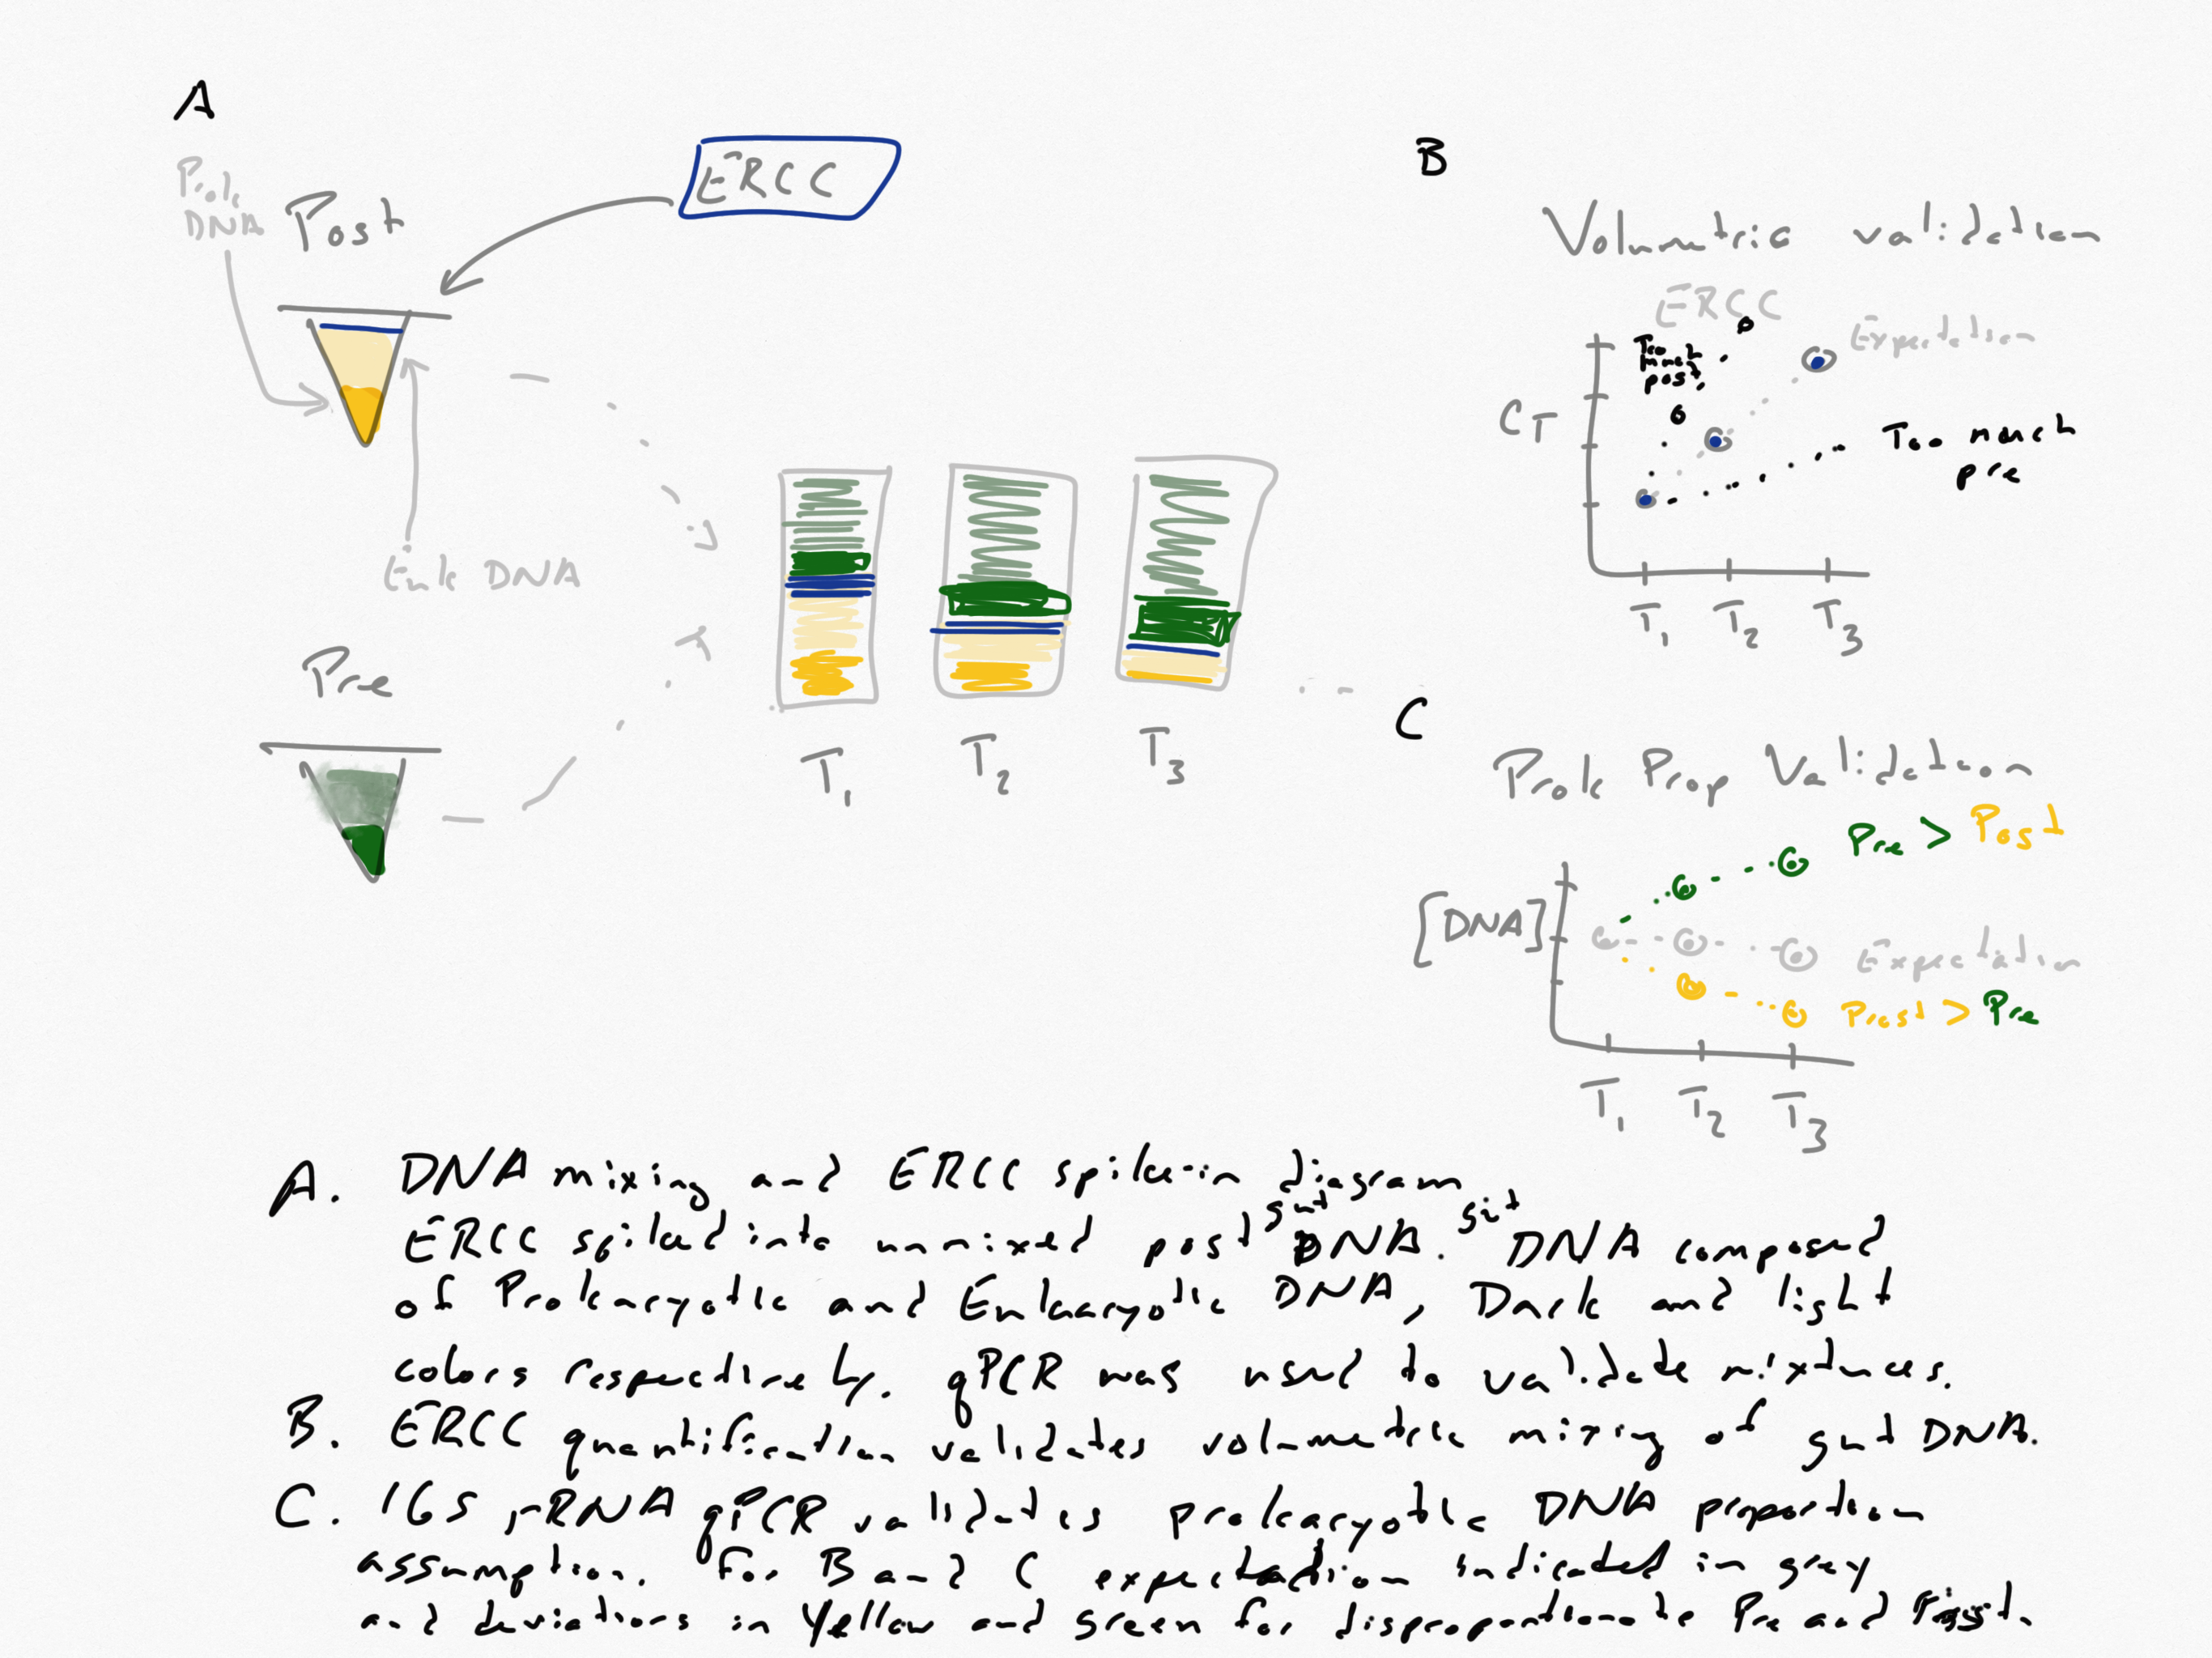
\includegraphics[width=0.9\linewidth]{titration_validation.png}
\caption{\label{fig:titrationValidation} Titration-series validation methods. (A) ERCCs were spiked into unmixed PRE and POST DNA. Unmixed DNA is composed of prokaryotic and eukaryotic DNA. The proportion of prokarytic DNA differs between PRE and POST resulting in the proportion of measureable PRE and POST DNA (prokarytic DNA) in the titrations differing from the mixture design. (B) Results from qPCR quantification of the ERCCs was used to validate volumetric mixing. (C) 16S rRNA qPCR is used to validate the prokaryotic DNA proportion. For B and C expectation is indicated in grey. Deviations from expectation along with explanations are indicated in black for B and yellow and green for C.}
\end{figure}

\paragraph*{Volumetric Mixing Validation}
Titration series volumetric mixing was validated using qPCR to quantify exogenous
DNA (ERCC plasmids) spiked into the POST samples prior to mixing.
The expectation is that the ERCC plasmid copy number will change at a rate consistent
with the change in proportion of POST along the titration series
(Main Fig. 1B and \ref{fig:titrationValidation}).
For our \(log_2\) two-sample-titration mixture design the expected slope of the
regression line between titration factor and Ct is 1, corresponding to a
doubling in template DNA every PCR cycle. The qPCR assay
standard curves had a high level of precision with \(R^2\) values close
to 1 and amplification efficiencies between 0.84 and 0.9 for all
standard curves indicating the assays were suitable for validating the
titration series volumetric mixing (Table \ref{tab:erccTable}). The qPCR assays targeting the
ERCCs spiked into the POST samples had \(R^2\) values and slope
estimates close to 1 (Table \ref{tab:erccTable}). Slope estimates less
than one were attributed to assay standard curve efficiency less than 1
(Table \ref{tab:erccTable}). When considering the
quantitative limitations of the qPCR assay these results confirm that
the unmixed samples were volumetrically mixed according to the
two-sample titration mixture design.

\begin{table}

\caption{\label{tab:erccTable}ERCC Spike-in qPCR assay information and summary statistics.
ERCC is the ERCC identifier for the ERCC spike-in, Assay is TaqMan assay, and Length
and GC are the size and GC content of the qPCR amplicon.  The Std. $R^2$ and Efficiency
(E) statistics were computed for the standard curves. $R^2$ and slope for titration qPCR results for the titration series.}
\centering
\resizebox{\linewidth}{!}{
\begin{tabular}[t]{lllrrrrr}
\toprule
Subject & ERCC & Assay & Length & Std. $R^2$ & E & $R^2$ & Slope\\
\midrule
E01JH0004 & 012 & Ac03459877-a1 & 77 & 0.9996 & 86.19 & 0.98 & 0.92\\
E01JH0011 & 157 & Ac03459958-a1 & 71 & 0.9995 & 87.46 & 0.95 & 0.90\\
E01JH0016 & 108 & Ac03460028-a1 & 74 & 0.9991 & 87.33 & 0.95 & 0.84\\
E01JH0017 & 002 & Ac03459872-a1 & 69 & 0.9968 & 85.80 & 0.89 & 0.93\\
E01JH0038 & 035 & Ac03459892-a1 & 65 & 0.9984 & 86.69 & 0.95 & 0.94\\
\bottomrule
\end{tabular}}
\end{table}


\begin{figure}
\centering
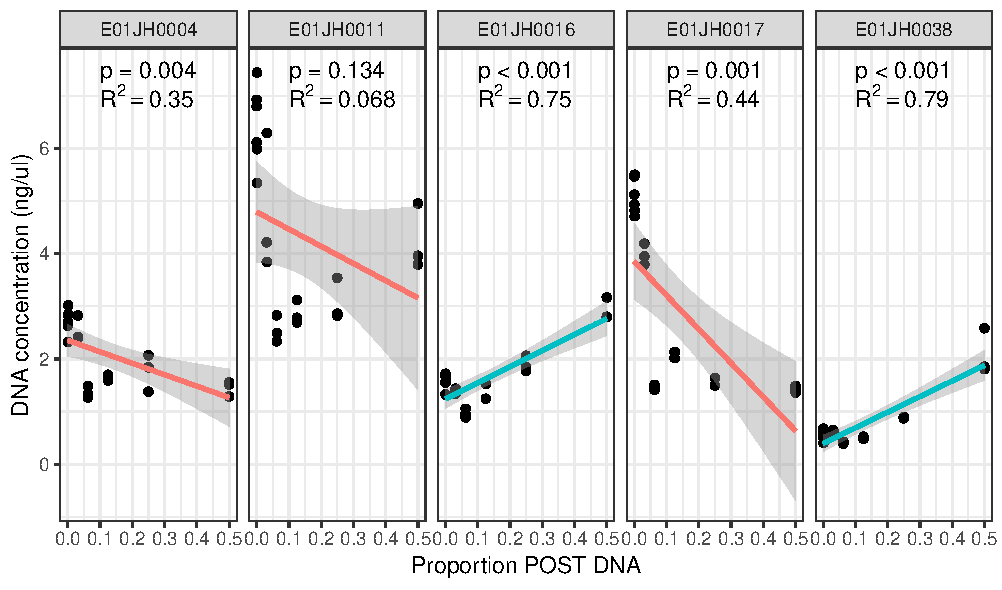
\includegraphics[width=0.9\linewidth]{bacPlot-1.pdf}
\caption{\label{fig:bacPlot}Prokaryotic DNA concentration (ng/ul) across
titrations measured using a 16S rRNA qPCR assay. \(R^2\) and p-values are linear
models fit to prokaryotic DNA concentration versus proportion post DNA for each individual.
Red and blue lines indicate negative and positive slope estimates respectively.
p-value indicates significant difference from the expected slope of 0.
The grey regions indicate the linear model 95\% confidence interval.
Multiple test correction was performed using the Benjamini-Hochberg
method. One of the E01JH0004 PCR replicates for titration 3
(\(\theta=0.125\)) was identified as an outlier, with a prokaryotic DNA
concentration of 0.003 ng/ul, and was excluded from the linear model.
The linear model slope was still significantly different from 0 when the
outlier was included.}
\end{figure}

\paragraph*{Prokaryotic DNA Proportion Validation}
Observed changes in prokaryotic DNA concentration across titrations
indicate the proportion of prokaryotic DNA from the unmixed PRE and POST
samples in a titration is inconsistent with the mixture design (Fig.
\ref{fig:bacPlot}). A qPCR assay targeting the 16S rRNA gene was used to
quantify the concentration of prokaryotic DNA in the titrations. If the
proportion of prokaryotic DNA is the same between PRE and POST samples
the slope of the concentration estimates across the two-sample titration
would be 0. For subjects where the proportion of prokaryotic DNA is
higher in the PRE samples, the slope will be negative, and positive when
the proportion is higher for POST samples. The slope estimates are
significantly different from 0 for all subjects excluding E01JH0011
(Fig. \ref{fig:bacPlot}). These results indicate that the proportion of
prokaryotic DNA is lower in POST when compared to the PRE samples for
E01JH0004 and E01JH0017 and higher for E01JH0016 and E01JH0038.


\paragraph*{Correcting for Deviations from Mixture Design}
%% Incorporate into text - only present unclustered
% The unclustered count table was generated using the
% 40,000 most abundant features from Mothur's initial pre-processing (see
% Methods for details).
% Unclustered pipeline \(\theta\) estimates were
% used to calculate the error rates for all pipelines to prevent
% over-fitting.

\begin{figure}
\centering
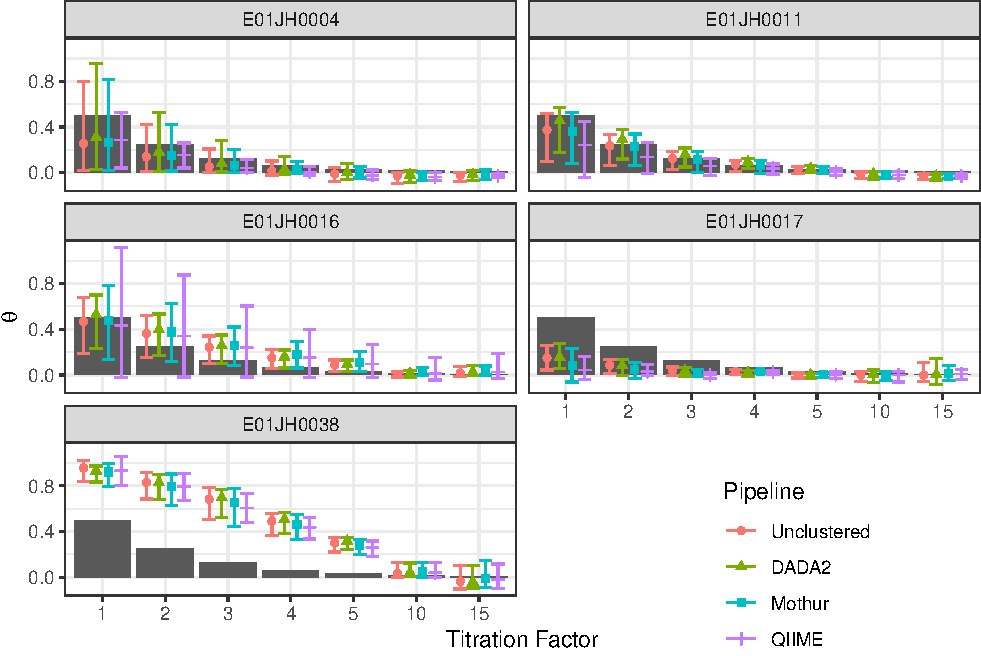
\includegraphics[width=0.9\linewidth]{thetaHat-1.pdf}
\caption{\label{fig:thetaHat}Theta estimates (\(\hat{\theta}\)) by titration, biological
replicate, and bioinformatic pipeline. Points indicate mean
of 1000 bootstrap \(\theta\) estimates and error bars 95\% confidence
interval. Grey bars indicate expected \(\theta\) values based on mixture design.
Points above grey bars indicate the titrations with a high proportion of prokaryotic DNA
from the POST sample than expected. Points below grey bars indicate titrations
with high proportion of prokaryotic DNA from the PRE sample.}
\end{figure}

Our titration validation results identified differences in the
proportion of prokaryotic DNA in PRE and POST samples (Fig. \ref{fig:bacPlot}).
Therefore our expected values used in measurement assessment need to account
for differences in the proportion of prokaryotic DNA from unmixed samples.
To account for differences in prokaryotic DNA proportion we inferred
the proportion of POST sample prokaryotic DNA in a titration, \(\theta\), using
the 16S rRNA sequencing data (Fig. \ref{fig:thetaHat}). Overall the relationship
between the inferred and mixture design \(\theta\) values were
consistent across pipelines but not subject whereas the \(\theta\)
estimate 95\% CI varied by both subject and pipeline. For study subjects
E01JH0004, E01JH0011, and E01JH0016 the inferred and mixture design
\(\theta\) values were in agreement, in contrast to study subjects
E01JH0017 and E01JH0038. For E01JH0017 the inferred values were
consistently less than the mixture design values. For E01JH0038
the inferred values were consistently greater than the mixture design
values. These results were consistent with the qPCR prokaryotic DNA
concentration results with significantly positive slopes for E01JH0004
and E01JH0016 and significantly negative slope for E01JH0038 (Fig.
\ref{fig:bacPlot}).

\clearpage

\begin{figure}
\centering
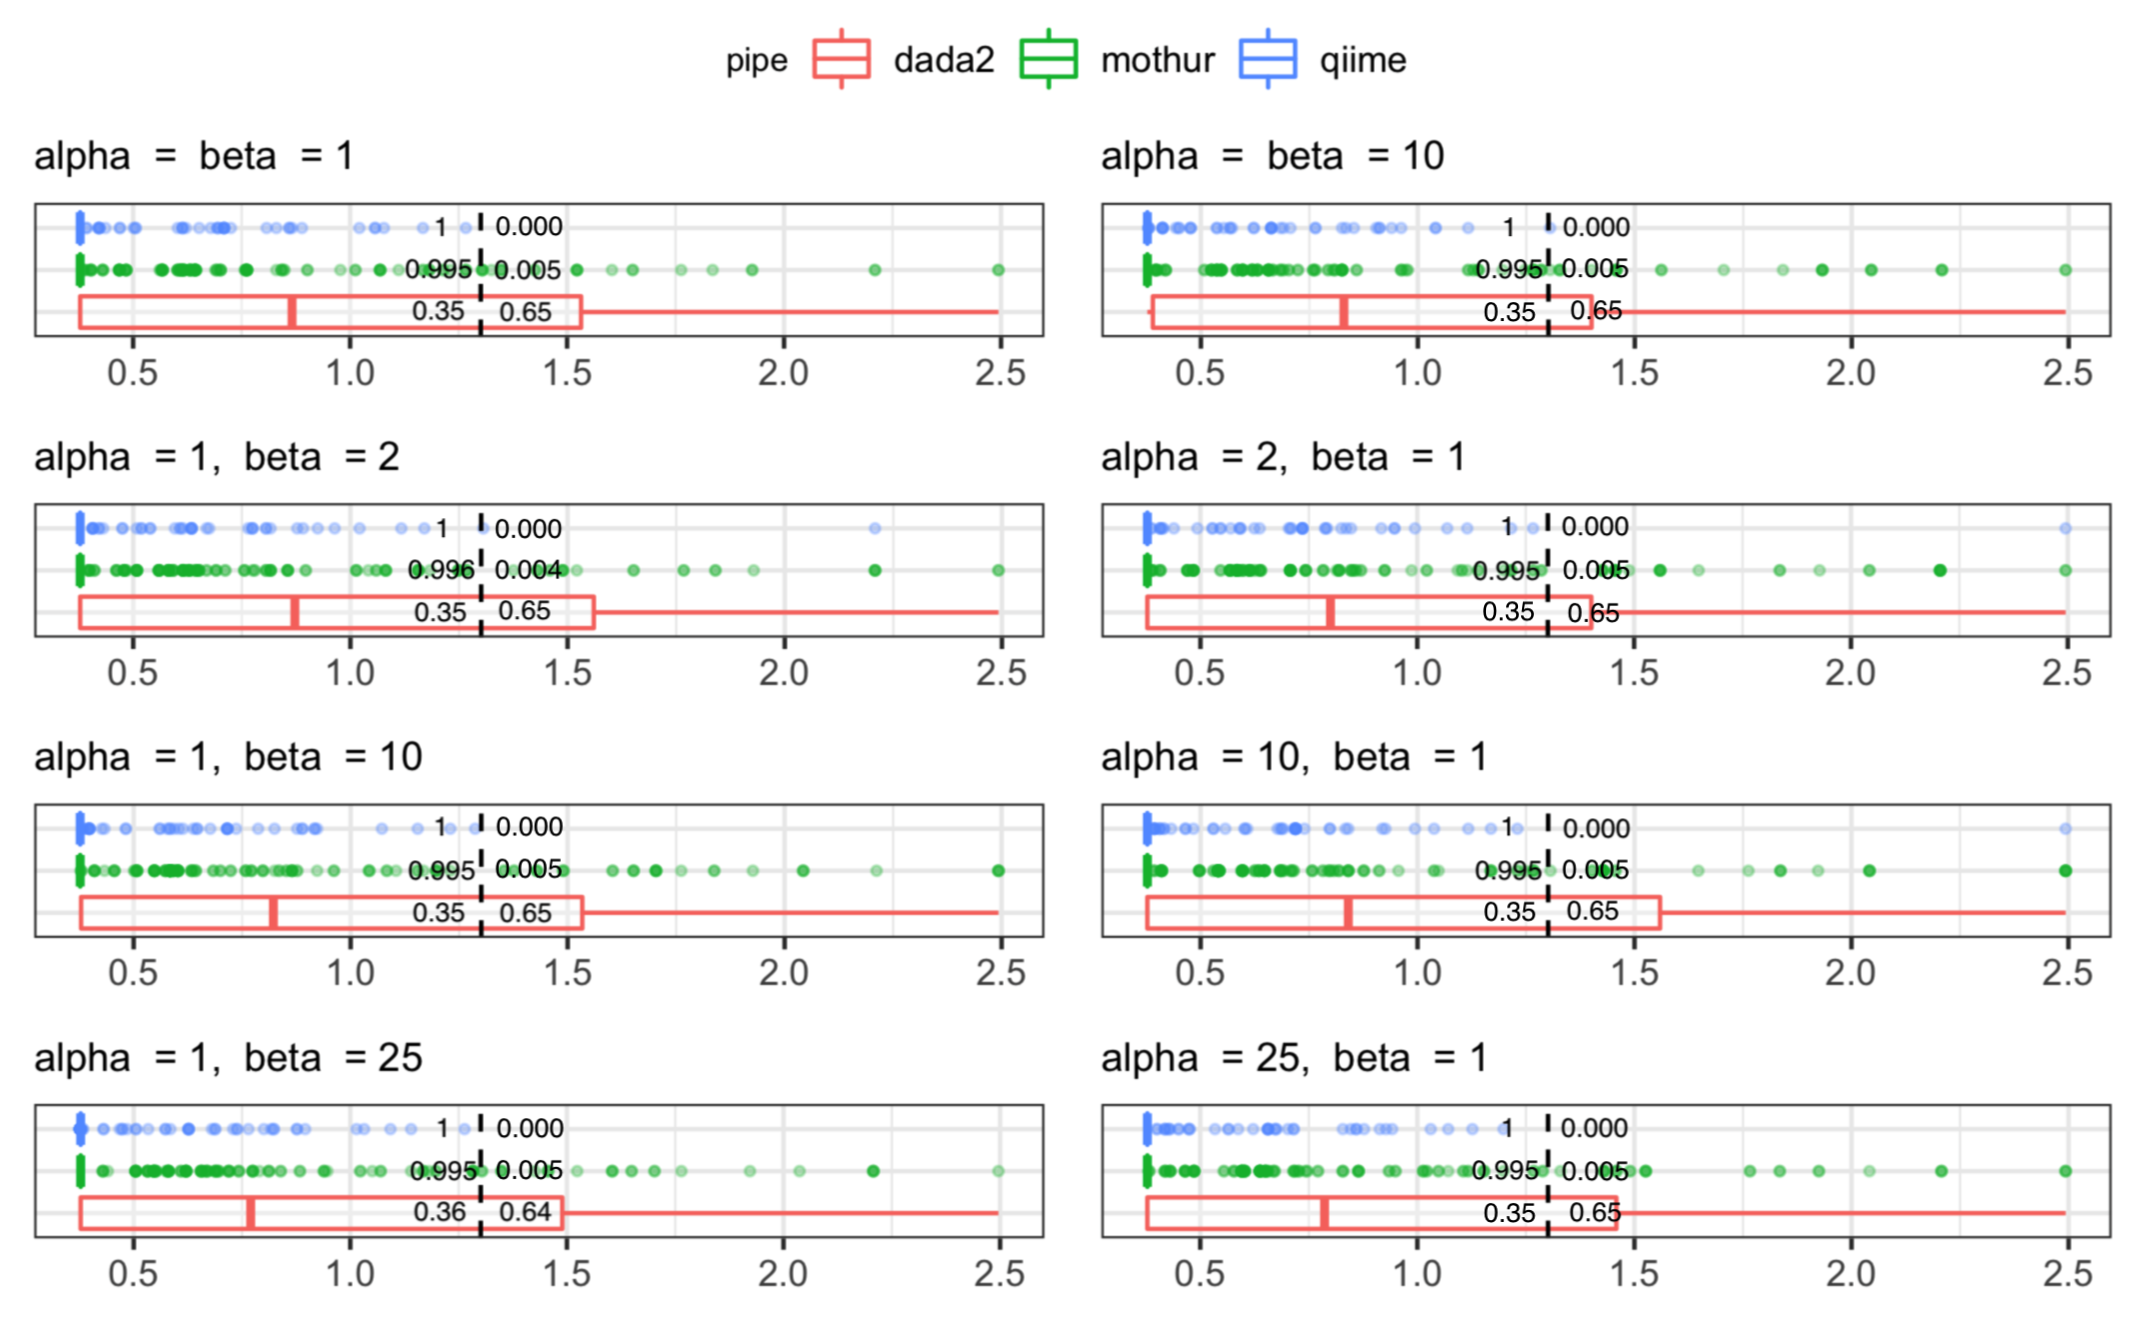
\includegraphics[width=0.9\linewidth]{bayes_beta.png}
\caption{\label{fig:bayesPrior} The x-axis of the plots above are -log10(adjusted p-value) for each titration-specific feature as calculated from equation (4) and the dotted black line indcates the value for -log10(0.05), our determined threshold for significance. Should a feature receive a p-value $<$ 0.05 (to the right of the dotted black line), then its detection as a titration-specific feature could not be explained due to sampling alone, and thus is an error of the computational pipeline. DADA2 is the only computational pipeline for which a large proportion of the titration-specific features could not be explained by sampling alone. The black text immediately to the left and right of the dotted black line are the proportions of titration-specific features which could and could not be explained by sampling error alone (respectively).}
\end{figure}

\section*{Bayesian Hypothesis Test - beta priors}
To test whether our choice of uniform prior was misrepresenting the distribution of feature abundance simulated from, we ran the Bayesian hypothesis test given in equations (3) and (4) using a beta prior distribution under various parameterizations of shape parameters alpha and beta (Fig. \ref{fig:bayesPrior}). By weighting the (beta) parameter higher, the sampling distribution simulated will skew left, with a higher chance of simulating a low or null count, as is customary in microbiome data. If the alpha parameter is weighted higher, then the sampling distribution is skewed right, towards higher abundant features and a long tail of lower abundant features. We found that no matter the choice of beta prior, the results of the hypothesis tests were consistent: DADA2 finds far more titration specific features that cannot be explained by sampling error alone and are likely the effects of clustering errors.

\cleardoublepage

\bibliographystyle{bmc-mathphys}
\bibliography{abundanceAssessment} 

\cleardoublepage

\section*{Supplemental Tables and Figures}
\clearpage

\begin{table}
\caption{\label{tab:sparsity}Sparsity levels for the three pipelines examined across all subjects (PRE and POST) and overall.}
\centering
\begin{tabular}[t]{lrrr}
\toprule
Subject   & DADA2 & Mothur & QIIME \\
\midrule
E01JH0004 & 0.69  & 0.74   & 0.50  \\
E01JH0011 & 0.74  & 0.78   & 0.60  \\
E01JH0016 & 0.72  & 0.77   & 0.57  \\
E01JH0017 & 0.65  & 0.71   & 0.45  \\
E01JH0038 & 0.71  & 0.79   & 0.66  \\
\midrule
Overall   & 0.93  & 0.98   & 0.94  \\
\bottomrule
\end{tabular}
\end{table}

\begin{table}
\caption{\label{tab:relAbuErrorTbl}Maximum feature-level error rate bias (median error rate) and variance (robust COV) by pipeline and individual.}
\centering
\resizebox{\linewidth}{!}{
\begin{tabular}[t]{llrrrrr}
\toprule
Metric & Pipeline & E01JH0004 & E01JH0011 & E01JH0016 & E01JH0017 & E01JH0038\\
\midrule
 & DADA2 & 2.37 & 2.55 & 17.03 & 4.34 & 0.66\\
\cmidrule{2-7}
 & Mothur & 5.30 & 6.76 & 19.24 & 4.15 & 1.93\\
\cmidrule{2-7}
 & QIIME & 3.99 & 6.43 & 8.83 & 4.80 & 1.09\\
\cmidrule{2-7}
\multirow{-4}{*}{\raggedright\arraybackslash Bias} & Unclustered & 6.45 & 7.24 & 16.85 & 4.37 & 1.91\\
\cmidrule{1-7}
 & DADA2 & 4.60 & 8.96 & 7.36 & 5.91 & 6.71\\
\cmidrule{2-7}
 & Mothur & 4.71 & 7.35 & 3.71 & 5.70 & 8.01\\
\cmidrule{2-7}
 & QIIME & 4.40 & 22.57 & 4.46 & 17.10 & 7.91\\
\cmidrule{2-7}
\multirow{-4}{*}{\raggedright\arraybackslash Variance} & Unclustered & 7.06 & 10.30 & 16.94 & 8.07 & 6.00\\
\bottomrule
\end{tabular}}
\end{table}

\begin{figure}
\centering
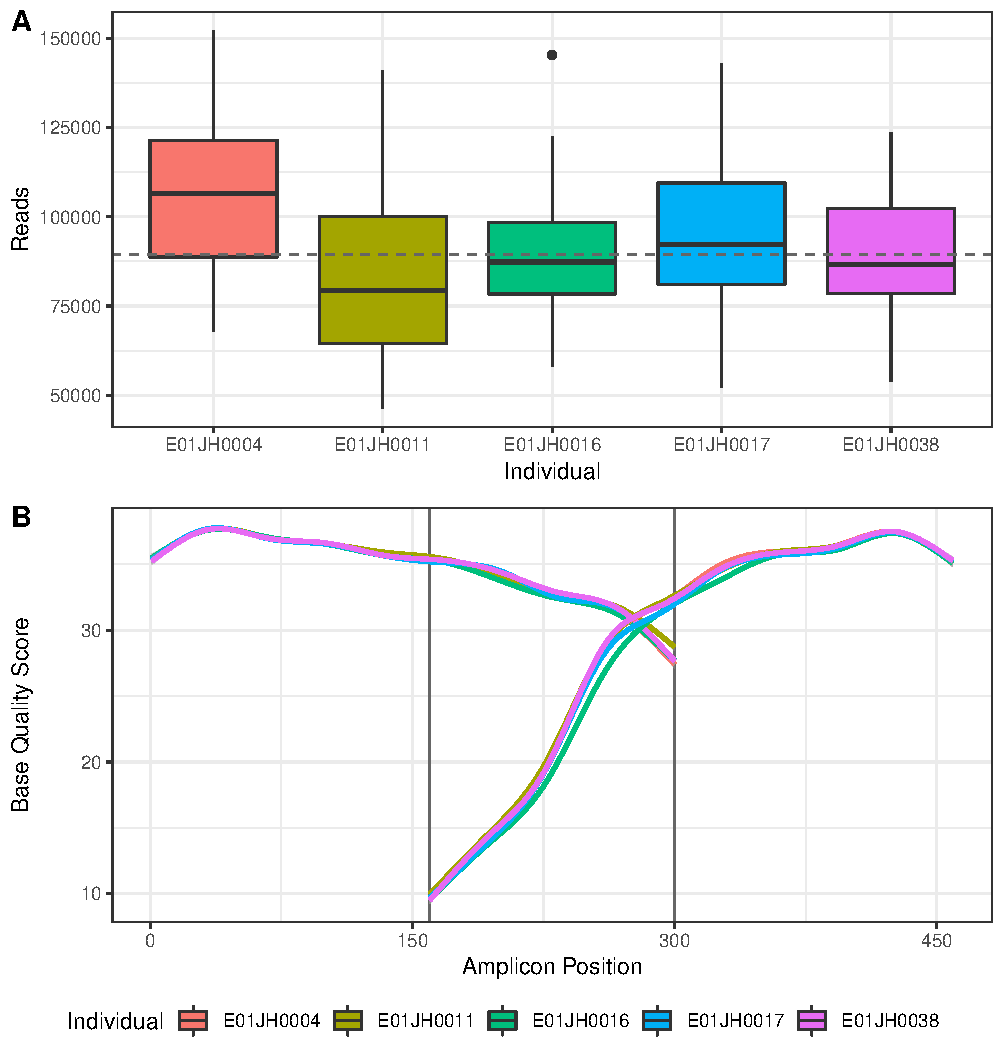
\includegraphics[width=0.9\linewidth]{qaPlots-1.pdf}
\caption{\label{fig:qaPlots}Sequence data set characteristics. (A)
Distribution in the number of raw reads generated per barcoded sample (Library Size)
by individual. Boxplots summarize data distribution with horizontal bar
as median, boxes indicating interquartile range, whiskers
\(\pm 1.5\times IQR\), and black points outliers. The dashed horizontal
line indicates overall median library size. Excluding one PCR replicate
from subject E01JH0016 titration 5 that had only 3,195 reads. (B)
Smoothing spline of the base quality score (BQS) across the amplicon by
subject. Vertical lines indicate approximate overlap region between
forward and reverse reads. Forward reads go from position 0 to 300 and
reverse reads from 464 to 164.
}
\end{figure}

\begin{figure}
\centering
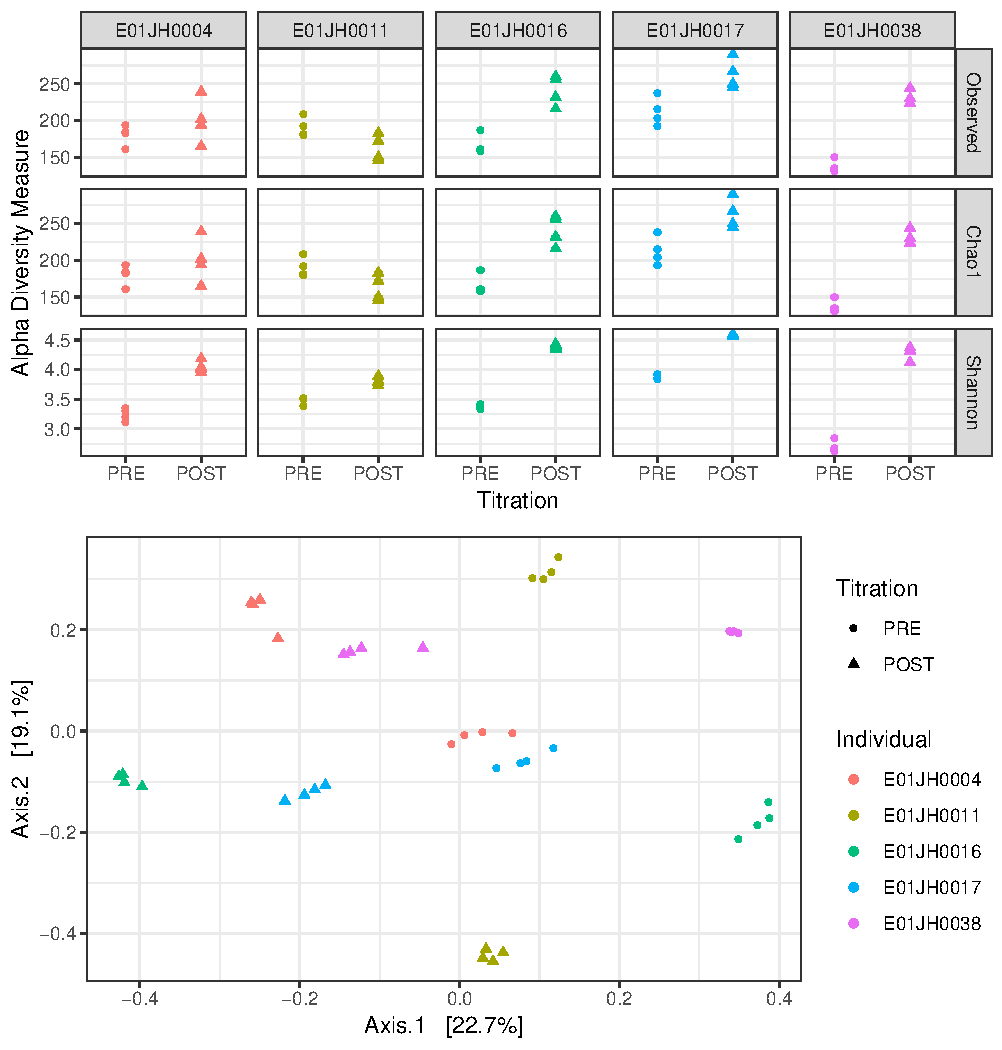
\includegraphics[width=0.9\linewidth]{sample_div.pdf}
\caption{\label{fig:sampleDiversity} Diversity metrics for PRE and POST samples by individual. 
Alpha (A) and Beta (B) diversity was calculated using the DADA2 count table. 
Beta-Diversity was calculated using Bray-Curtis diversity metric and principal components analysis was used for ordination. The same color and shape scale was used for plots A and B.}
\end{figure}

\begin{figure}
\centering
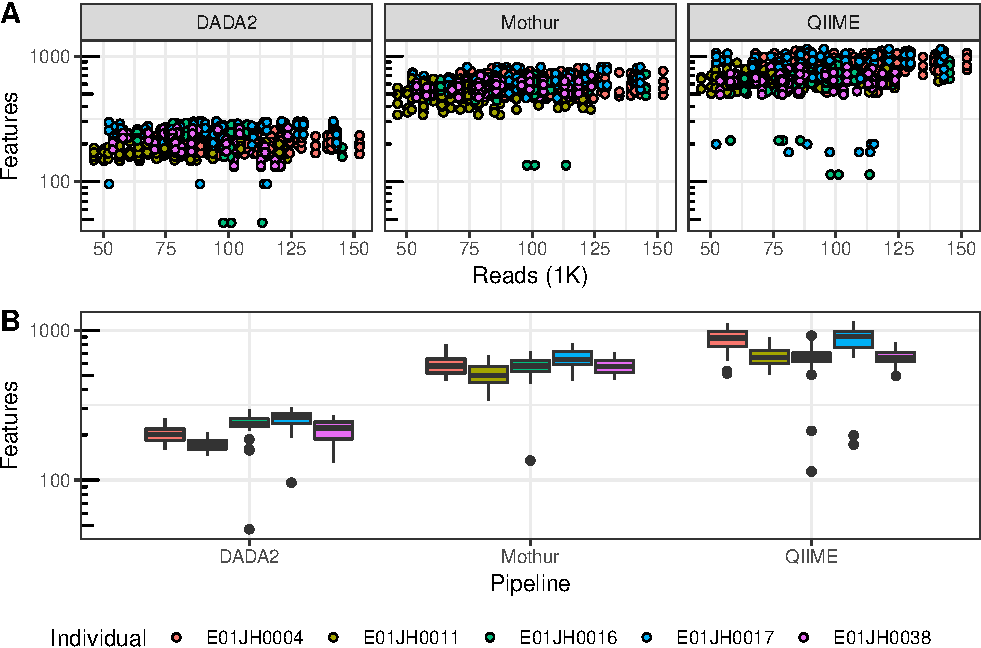
\includegraphics[width=0.9\linewidth]{readsVfeats-1.pdf}
\caption{\label{fig:readsVfeats}Relationship between the number of reads and
features per sample by bioinformatic pipeline. (A) Scatter plot of
observed features versus raw reads per sample. (B) Observed
feature distribution by pipeline and individual. Excluding one PCR
replicate from subject E01JH0016 titration 5 with only 3,195 reads, and
the Mothur E01JH0017 titration 4 (all four PCR replicates), with 1,777
observed features.}
\end{figure}

\begin{figure}
\centering
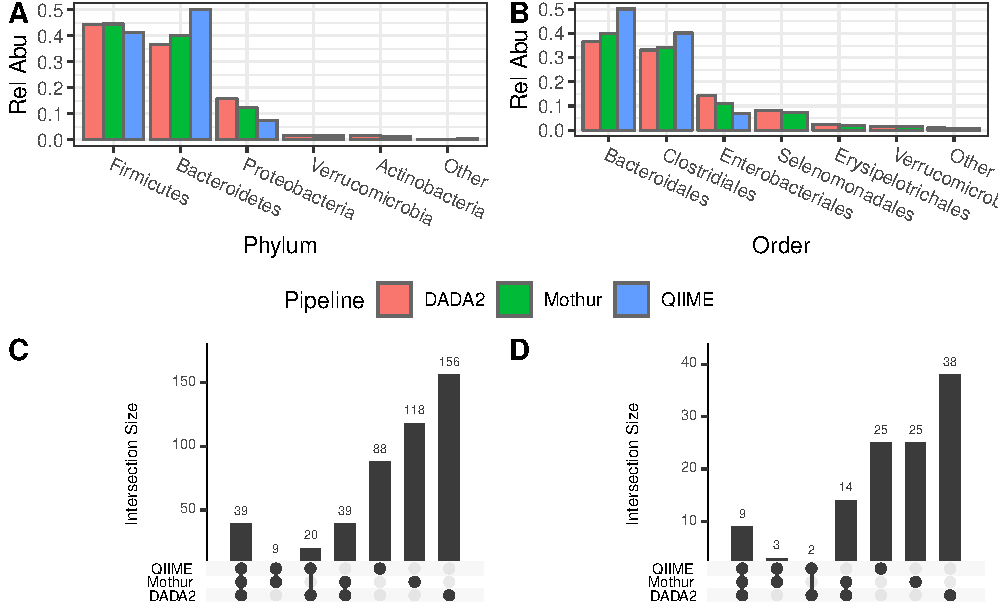
\includegraphics[width=0.9\linewidth]{pipeTaxa-1.pdf}
\caption{\label{fig:pipeTaxa} Comparison of dataset taxonomic composition
across pipelines. Phylum (A) and Order (B) relative abundance by
pipeline. Taxonomic groups with less than 1\% total relative abundance
were grouped together and indicated as other. Pipeline genus-level
taxonomic assignment set overlap for all genera (C) and the upper
quartile genera by relative abundance for each pipeline (D). Intersection size is
the number of features observed in the pipeline combination indicated on the x-axis.
For example in C, 39 genera are observed in all three pipelines and
88 are observed in only QIIME and not Mothur or DADA2.}
\end{figure}

\begin{figure}
\centering
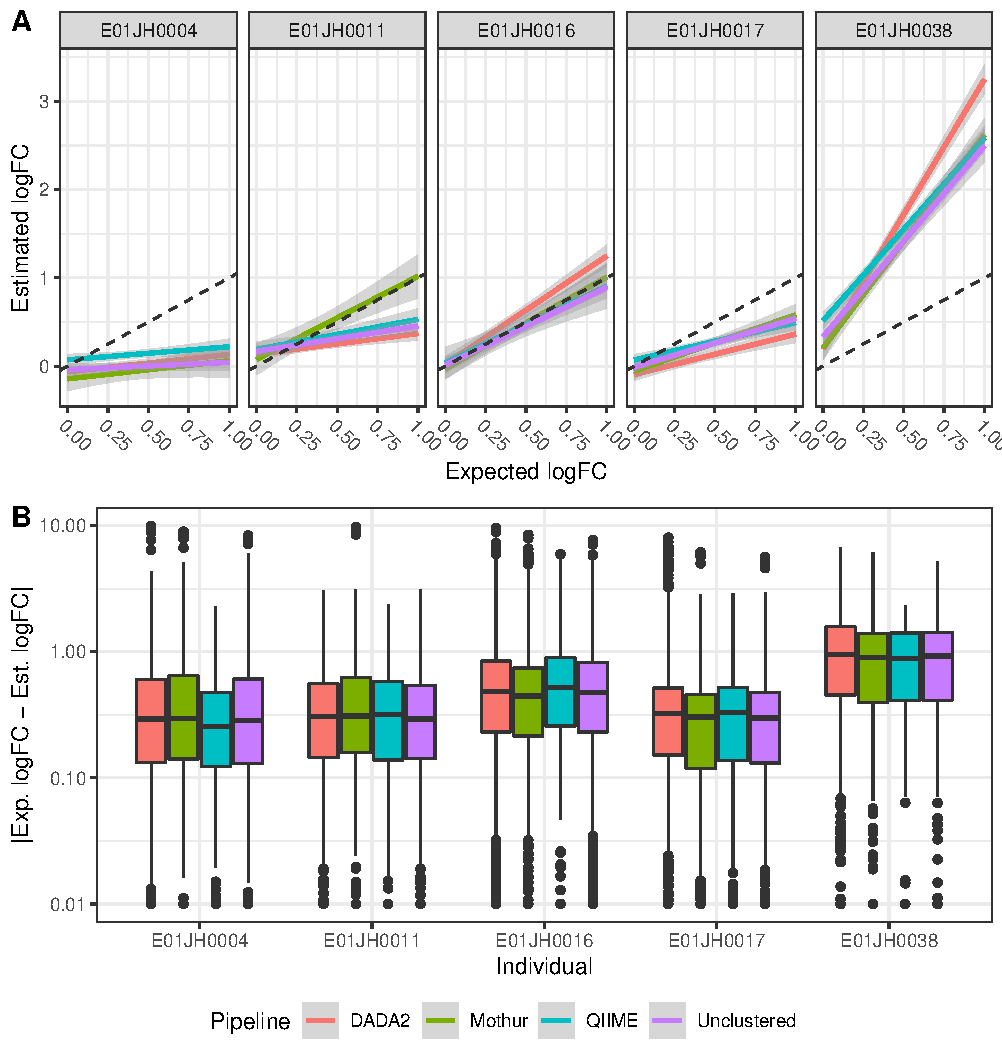
\includegraphics[width=0.9\linewidth]{logFCerror-1.pdf}
\caption{\label{fig:logFCerror} Differential abundance quantitative assessment. (A) Linear model of the relationship between
estimated and expected log fold-change relative abundance between titrations for PRE-specific and
PRE-dominant features by pipeline and individual, line color indicates
pipelines. Dashed grey line indicates expected 1-to-1 relationship
between the estimated and expected log fold-change. (B) Log fold-change
error (\textbar{}exp-est\textbar{}) distribution by pipeline and
individual.}
\end{figure}

\begin{figure}
\centering
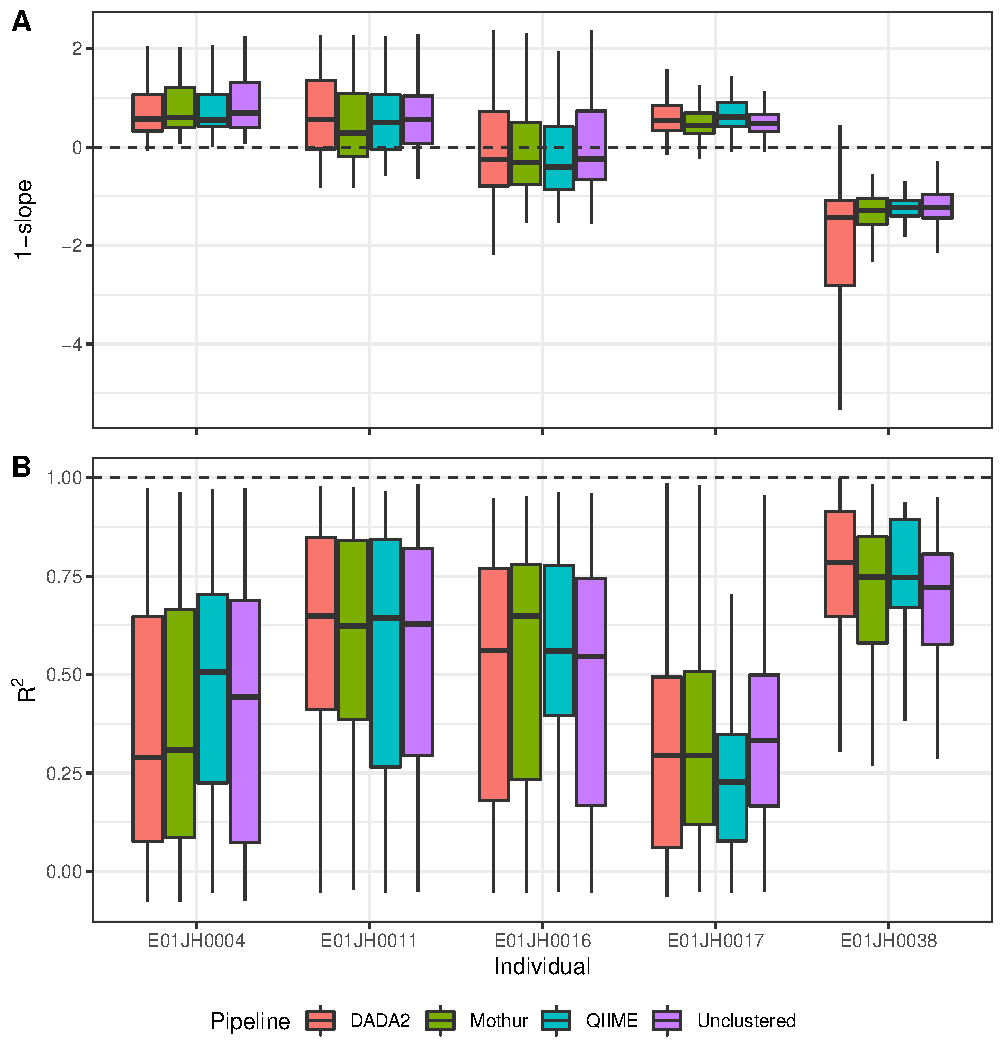
\includegraphics[width=0.9\linewidth]{logFcErrorMetrics-1.pdf}
\caption{\label{fig:logFcErrorMetrics}Feature-level differential abundance assessment.
Log-fold change error
bias (A) and variance (B) metric distribution by subject and pipeline.
The bias (\(1 - slope\)) and variance (\(R^2\)) metrics are derived from
the linear model fit to the estimated and expected log fold-change
values for individual features. Boxplot outliers, \(1.5\times IQR\) from
the median were excluded from the figure to prevent extreme metric
values from obscuring metric value visual comparisons.}
\end{figure}

\end{document}